\documentclass{article}[11pt]
\usepackage[frenchb,english]{babel}
\usepackage[T1]{fontenc}
\usepackage[utf8]{inputenc}
\usepackage{amsmath,amssymb,latexsym}
\usepackage{times}
\usepackage{float}
\usepackage[left=2cm,right=2cm,top=2cm,bottom=2cm]{geometry}
\frenchbsetup{StandardLists=true} % � inclure si on utilise \usepackage[french]{babel}
\usepackage{enumitem}
\usepackage{fancyhdr}
\usepackage{mathrsfs}
\usepackage{graphicx}
%\usepackage[Algorithme]{algorithm}
%\usepackage{algorithmic}
\usepackage{tikz}
\usepackage{tabularx}
\usetikzlibrary{shapes}
\pagestyle{fancy}
\newcommand{\tr}[1]{{\vphantom{#1}}^{\mathit t}{#1}} 
\renewcommand\headrulewidth{1pt}
\fancyhead[L]{Cours 1�re S}
\fancyhead[R]{Yoann Pietri}
\newcounter{theoremecounter}[subsection]
\usepackage{titlesec}
\setcounter{secnumdepth}{3}% enl�ve la num�rotation apr�s les sections
%\renewcommand\thechapter {\Roman{chapter}}

 \setlength{\parindent}{0pt}

\newcommand{\R}{\mathbb{R}}
\newcommand{\N}{\mathbb{N}}
\newcommand{\Q}{\mathbb{Q}}
\newcommand{\Z}{\mathbb{Z}}
\newcommand{\C}{\mathbb{C}}
\newcommand{\K}{\mathbb{K}}
\newcommand{\eqi}{\Leftrightarrow}
\titleformat{\subsubsection}
   {\normalfont\fontsize{11pt}{13pt}\selectfont\bfseries}% apparence commune au titre et au num�ro
   {\thesubsubsection}% apparence du num�ro
   {1em}% espacement num�ro/texte
   {}% apparence du titre

\tikzstyle{theobox} = [draw=black, very thick,
    rectangle, rounded corners, inner sep=10pt, inner ysep=20pt]
\tikzstyle{theotitle} =[fill=white, text=black,rounded corners,draw=black,very thick]

\fancyhead[L]{Contrôle chapitre 8}

\usepackage[c]{esvect}
\newcommand{\covec}[2]{\begin{pmatrix}#1 \\#2 \end{pmatrix}}

\begin{document}
\center
\Large Contrôle de cours
\flushleft
\center
Statistiques
\flushleft \normalsize
Durée du contrôle : 1h\newline
Ce sujet comporte 2 pages\newline
La calculatrice est autorisée
\subsection*{Exercice 1 (R.O.C., temps conseillé : 10 min) : }
La variance d'une série statistique se calcule par 
$$\frac{1}{n}\sum_{i=1}^n (x_i - \overline{x})^2 n_i$$
Pour obtenir la formule de König-Huygens, on développe le carré : 
$$\frac{1}{n}\sum_{i=1}^n (x_i - \overline{x})^2 n_i =\frac{1}{n}\sum_{i=1}^n (x_i^2 -2x_i\overline{x} + \overline{x}^2) n_i = $$
$$\frac{1}{n}\sum_{i=1}^n (x_i - \overline{x})^2 n_i =\frac{1}{n}(\sum_{i=1}^n x_i^2n_i -\sum_{i=1}^n 2x_i\overline{x}n_i + \sum_{i=1}^n\overline{x}^2 n_i$$
$$V(x) =\overline{x^2} -2\overline{x}^2 + \overline{x}^2$$
$$V(x) =\overline{x^2} -\overline{x}^2$$
\subsection*{Exercice 2 (Caractère discret, temps conseillé : 15 min) : }
\begin{enumerate}
\item Le caractère prend ici un nombre fini de valeurs (il ne prend pas ses valeurs dans un intervalle)
\item L'effectif total de cette série statistique est $10 + 8 + 7 + 3 + 2 + 3 + 5 + 9 +11 +13 +15 = 86$ $$\boxed{n=86}$$ 
\item Voici le tableau des fréquences\newline
\begin{tabularx}{\linewidth}{|X|X|X|X|X|X|X|X|X|X|X|X|}
\hline
N (*) & 0 & 1 & 2 & 3 & 4 & 5 & 6 & 7 & 8 & 9 & 10\\ \hline
Fréqu-
ence & $\frac{10}{86}$ & $\frac{8}{86}$ & $\frac{7}{86}$ & $\frac{3}{86}$ & $\frac{2}{86}$ & $\frac{3}{86}$ & $\frac{5}{86}$ & $\frac{9}{86}$ & $\frac{11}{86}$ & $\frac{13}{86}$ & $\frac{15}{86}$ \\ \hline
\end{tabularx}\newline
et on peut donner valeurs approchées \newline
\begin{tabularx}{\linewidth}{|X|X|X|X|X|X|X|X|X|X|X|X|}
\hline
N (*) & 0 & 1 & 2 & 3 & 4 & 5 & 6 & 7 & 8 & 9 & 10\\ \hline
Fréqu-
ence & $0,1162$ & $0,0930$ &$0,0814$ & $0,0348$ & $0,0232$ & $0,0348$ & $0,0581$ & $0,1046$ & $0,1279$ & $0,1512$ & $0,1748$ \\ \hline
\end{tabularx}\newline
\item On donne des valeurs approchées (calcul non détaillés) : 
$$\boxed{\overline{x} = 5,84}$$
$$\boxed{Me = Q_2 = 7}$$
$$\boxed{Q_1 = 2}$$
$$\boxed{Q_3 = 9}$$
$$\boxed{Q_3 - Q_1 = 7}$$
$$\boxed{e = 10-0 = 10}$$
$$\boxed{v(x) = 13,03}$$
$$\boxed{\sigma = 3,61}$$
L'écart inter-quartiles (resp. la variance et l'écart type) servent à mesurer les écarts à la médiane (resp. la moyenne). La médiane coupe la série en deux : il a autant d'élèves qui ont validé plus de 7 capacités que d'élèves qui ont validé moins de 7 et les quartiles coupent la série en 4
\item Histogramme de la série : \newline
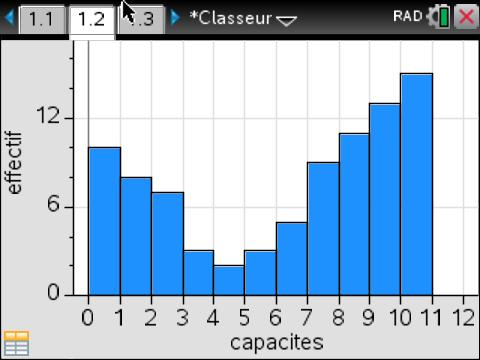
\includegraphics[scale=0.5]{chap8_corr_ill1.jpg}\newline
Diagramme en boîte \newline
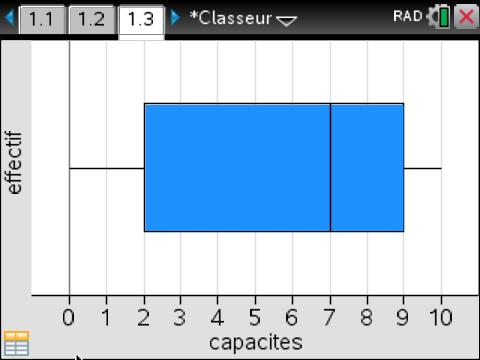
\includegraphics[scale=0.5]{chap8_corr_ill2.jpg}\newline
Diagramme circulaire\newline
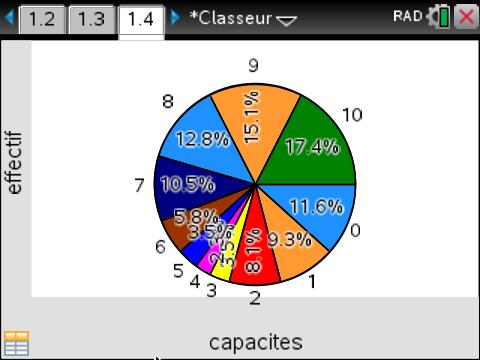
\includegraphics[scale=0.5]{chap8_corr_ill3.jpg}\newline
\item L'histogramme permet déjà d'avoir une idée de pourquoi on parle d'élèves hétérogènes. De plus un important écart-interquartiles devant la médiane et un important écart-type devant la moyenne assure une répartition vers les notes extrêmes.
\end{enumerate}
\subsection*{Exercice 3 (Caractère continu, temps conseillé : 15 min) : }
\begin{enumerate}
\item Pour la première série, on utilise la fait que la somme des effectifs doit être égal à l'effectif total. Pour le deuxième, on utilise la fait que la somme des fréquences est égale à 1 : ainsi les coefficients à compléter sont 
$$\boxed{212}$$
$$\boxed{0,0641}$$
\item Les résultats sont approchés : 
$$\boxed{\overline{x} = 11,94}$$
$$\boxed{Q_1 = 10}$$
$$\boxed{M_e = Q_2 = 12}$$ 
$$\boxed{Q_3 = 14}$$
$$\boxed{Q_3-Q_1 = 4}$$
$$\boxed{e = 30}$$
$$\boxed{V(x) = 19}$$
$$\boxed{\sigma =4,36}$$
Histogramme : \newline
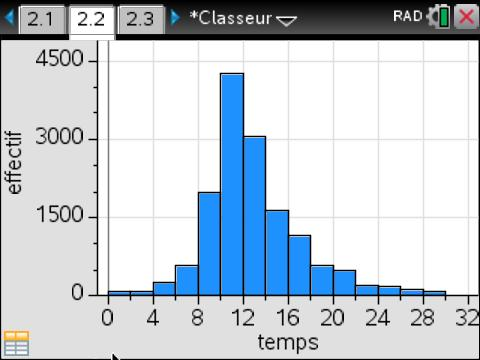
\includegraphics[scale=0.5]{chap8_corr_ill4.jpg}\newline
Diagramme en boite\newline
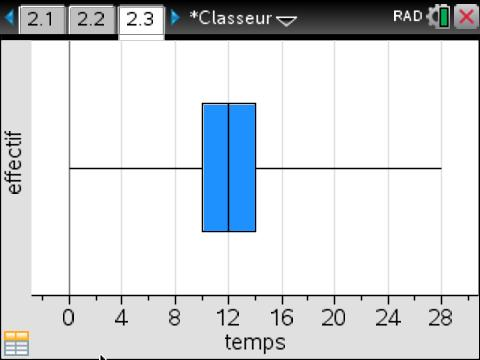
\includegraphics[scale=0.5]{chap8_corr_ill5.jpg}\newline
\item Les résultats sont approchés 
$$\boxed{\overline{x} = 16,32}$$
$$\boxed{\sigma = 4,23}$$
\item En moyenne, les jeunes entre 18 et 25 ans passent plus de temps sur internet. Remarquons un faible écart de l'écart type entre les 2 séries : les jeunes se répartissent de la même manière autour de leur moyenne
\end{enumerate}
\subsection*{Exercice 4 (Quelques nouveaux outils, temps conseillé : 20 min) : }

\begin{enumerate}
\item Les résultats sont approchés
$$\boxed{\overset{\circ}{x} = 0.99892}$$
$$\boxed{\overset{\sim}{e} = 0,00792}$$
$$\boxed{C_V = 36,5}$$
$$\boxed{\lambda_x = -0,0129}$$
$$\boxed{Y_x = 0}$$
$$\boxed{\mathscr{F}_x = 0,04}$$
\item Moyenne géométrique : autre moyen de faire la moyenne. \newline Ecart arithmétique : calcule l'écart à la moyenne; assimilable à l'écart type\newline Critère de dispersion : sert à voir l'étalement de la série en comparant l'écar type devant la moyenne (la multiplication par 100 est pour faire ressembler ça à un pourcentage) \newline Critère d'asymétrie de Pearson : quantifie l'asymétrie en comparant la moyenne et la médiane : dans le cas de série statistique symétrique, la moyenne est égale à la médiane et le coefficient est alors nul \newline Coefficient de Yule : quantifie les écarts entres quartiles et médiane \newline Coefficient d'aplatissement de Yule : il faut voir ça avec un histograme je pense
\item Pour tout $a$ et $b$, on a
$$(a-b)^2 \geq 0$$
$$a^2 - 2ab + b^2 \geq 0$$
$$a^2 - 2ab + b^2 +4ab \geq 4ab$$
$$a^2 + 2ab + b^2 \geq 4ab$$
$$(a+b)^2 \geq 4ab$$
$$a+b \geq 2 \sqrt{ab}$$
$$\frac{a+b}{2} \geq \sqrt{ab}$$ 
\end{enumerate}
$$\star \star \star$$
\center
FIN DU SUJET
\end{document}